\section{机器人操作系统(ROS)简介}
ROS(机器人操作系统,\underline{R}obot \underline{O}perating \underline{S}ystem)源于2007年斯坦福大学机器人实验室与  Willow Garage公司联合开发的开源项目,是专为机器人软件开发所设计出来的一套电脑操作系统架构。它是一个开源的元级操作系统(后操作系统),提供一系列面向机器人开发的硬件抽象、底层设备控制、节点(进程)间消息传递等功能\cite{fairchildROSRoboticsExample2016}。经过十多年的发展,ROS得到了科研人员的广泛关注,目前基于ROS开发的机器人包括TurtleBot、AscTec Pelican、Schunk LWA 4D等(图\ref{figure_ros_support})。
\begin{figure}[htbp]
  %\vspace{13pt}
  \centering
  \subfigure[TurtleBot]{
  \includegraphics[height=0.21\linewidth]{images/ch03/Inkedturtlebot.jpg} \label{figure_turtlebot}
  }\hspace{10pt}
  \subfigure[AscTec Pelican]{
  \includegraphics[height=0.21\linewidth]{images/ch03/asctec.jpg} \label{figure_asctec}
  }\hspace{10pt}
  \subfigure[Schunk LWA 4D]{
  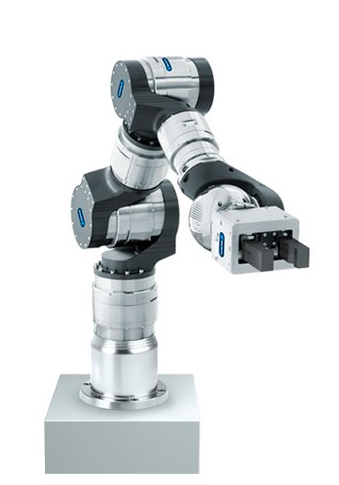
\includegraphics[height=0.21\linewidth]{images/ch03/lwa.png} \label{figure_lwa}
  }
  \caption{部分支持ROS的机器人}\label{figure_ros_support} % label 用来在文中索引
\end{figure}

分布式计算是ROS的典型特征,在ROS中机器人系统往往依赖多个计算机同时运行的多个节点,例如\cite{okaneGentleIntroductionROS2014}:
\begin{enumerate}[leftmargin=0em, listparindent=2em, parsep=0em, topsep=0em, label=(\theenumi)]
%\setlength{\leftmargin}{0em}
\setlength{\itemindent}{4em}
\setlength{\labelsep}{0em}
\setlength{\labelwidth}{2em}
\setlength{\parsep}{0em}
\setlength{\itemsep}{0em}
\setlength{\topsep}{0em}
%\setlength{\listparindent}{2em}
  \item 一些机器人搭载有多台计算机,每台计算机用于控制机器人的部分驱动器或传感器。
  \item 即使只有一台计算机, 通常仍将程序划分为独立运行且相互协作的小的模块来完成复杂的控制任务,这也是常见的做法。
  \item 当多个机器人需要协同完成一个任务时,往往需要互相通信来支撑任务的完成。
  \item 用户通常通过台式机、 笔记本或者移动设备发送指令控制机器人,这种人机交互接口可以认为是机器人软件的一部分。
\end{enumerate}

为满足上述要求,ROS提供了消息和服务两种相对简单并且完备的机制进行单计算机或多计算机不同进程间的通信。除此以外,标准包(Standard Packages)和通信接口使得现有算法可以快速移植到不同系统。事实上,随着机器人研究和机器人操作系统的快速发展,它已经集成了一批用于机器人建图、导航和路径规划等任务的算法。同时,其松耦合的结构设计使得机器人开发调试更加便捷和高效。上述原因使得ROS逐渐成为机器人软件领域的事实标准。本文使用ROS作为行为交互仿真平台的控制核心。

Gazebo是一个基于物理仿真的跨平台3D机器人模拟器软件,能够在复杂的环境中准确地模拟单个或多个机器人的运动,其对ROS的支持十分优秀,因此成为ROS开发者使用的主流仿真工具。目前,Gazebo已支持多种高性能的物理引擎,如ODE、Bullet、SimBody、DART等。经过简单的设置,用户即可向机器人添加传感器和自定义插件,并可添加传感器噪声。本文将利用Gazebo可视化仿生机器鼠交互时的场景。